%
%  Vincent Yannello
%
\documentclass[12pt,fullpage]{article}
\usepackage{fullpage}
\usepackage{amsmath}
\DeclareMathOperator{\erf}{erf}
\usepackage{psfrag}                                          % LaTeX graphics tool
\usepackage{pslatex}                                         % avoids the default cmr font
\usepackage{graphicx}                                        % graphics package 
\usepackage{epsfig}                                          % figures
\usepackage{hyperref}
\usepackage{color}

\begin{document}

\noindent
{\bf Logistic-exponential distribution} (from \color{blue}\url{http://www.math.wm.edu/~leemis/chart/UDR/UDR.html}\color{black})

\noindent
The shorthand $X \sim \hbox{logistic-exponential}(\alpha, \beta)$ is used to indicate that the
random variable $X$ has the logistic-exponential distribution with positive scale parameter $\alpha$ and
positive shape parameter $\beta$.
A logistic-exponential random variable $X$ with parameters $\alpha$ and $\beta$ has probability density function 
$$
f(x) = {\frac {{\it \kern 0.08 em \alpha}\,{\it \beta}\, \left( {e^{{\it \kern 0.08 em \alpha}\,x
}}-1 \right) ^{{\it \beta}-1}{e^{{\it \kern 0.08 em \alpha}\,x}}}{ \left( 1+ \left( {e
^{{\it \kern 0.08 em \alpha}\,x}}-1 \right) ^{{\it \beta}} \right) ^{2}}} \qquad \qquad x > 0,
$$
for all $\alpha > 0$ and for $\beta >0$. 
The probability density function for two different parameter settings is illustrated below.
{\begin{figure}[h!]
\begin{center}
\psfrag{lab1}{$\alpha \kern -0.08 em = \kern -0.08 em  5,\, \beta \kern -0.08 em  = \kern -0.08 em  1$}
\psfrag{lab2}{$\alpha \kern -0.08 em  = \kern -0.08 em  1,\, \beta \kern -0.08 em  = \kern -0.08 em  2$}
\psfrag{labx}{$x$}
\psfrag{labf}{$f(x)$}
\includegraphics[width=3.2in]{LogisticexponentialPlot.ps}
\end{center}
\end{figure}}\\
The cumulative distribution function on
the support of $X$ is
$$
F(x) = P(X \le x) = {\frac { \left( {e^{{\it \kern 0.08 em \alpha}\,x}}-1 \right) ^{{\it \beta}
}}{1+ \left( {e^{{\it \kern 0.08 em \alpha}\,x}}-1 \right) ^{{\it \beta}}}}  \qquad \qquad x > 0.
$$
The survivor function on the support of $X$ is
$$
S(x) = P(X \ge x) = \frac{1}{1+ \left( {e^{{\it \kern 0.08 em \alpha}\,x}}-1 \right) ^{{\it 
\beta}}}  \qquad \qquad x > 0.
$$
The hazard function on the support of $X$ is
$$
h(x) = {\frac {{\it \alpha}\,{\it \beta}\, \left( {e^{{\it \kern 0.08 em \alpha}\,x
}}-1 \right) ^{{\it \beta}-1}{e^{{\it \kern 0.08 em \alpha}\,x}}}{1+ \left( {e^{{\it 
\kern 0.08 em \alpha}\,x}}-1 \right) ^{{\it \beta}}}} \qquad \qquad x > 0.
$$
The cumulative hazard function on the support of $X$ is mathematically intractable.
$$
H(x) = \ln  \left( 1+ \left( {e^{{\it \kern 0.08 em \alpha}\,x}}-1 \right) ^{{
\it \beta}} \right) \qquad \qquad x > 0.
$$
The inverse distribution function of $X$ is
$$
F ^ {-1}(u) = \ln  \left(  \left( {\frac {u}{1-u}} \right) ^{1/\beta}+1 \right)\Big/\alpha \qquad \qquad 0 < u < 1.
$$
The median of $X$ is
$$
\frac{\ln(2)}{\alpha}.
$$
The moment generating function and characteristic function of $X$ are mathematically intractable. The population mean, variance, skewness, and kurtosis of $X$ are also mathematically intractable.

\vspace{0.1in}

\noindent
{\bf APPL verification:}
The APPL statements
\begin{verbatim}
X := [[x -> alpha * beta * (exp(alpha * x) - 1) ^ (beta - 1) * exp(alpha * x)/
            (1 + (exp(alpha * x) - 1) ^ beta) ^ 2],[0, infinity],
            ["Continuous", "PDF"]];
CDF(X);
SF(X);
HF(X);
CHF(X);
IDF(X);
\end{verbatim}
verify the cumulative distribution function, survivor function, hazard function, cumulative hazard function, and inverse distribution function.
\end{document}
